%%% Template for documenting projects which involve circuit illustrations and code.
% Author: Claudiu Groza

% Template based on the template created by:
% Author:   Luis José Salazar-Serrano
%           totesalaz@gmail.com / luis-jose.salazar@icfo.es
%           http://opensourcelab.salazarserrano.com


\documentclass[a4paper,11pt]{article}

\usepackage[T1]{fontenc}
\usepackage[utf8]{inputenc}
\usepackage{graphicx}
\usepackage{xcolor}

\renewcommand\familydefault{\sfdefault}
\usepackage{tgheros}
\usepackage[defaultmono]{droidmono}

\usepackage{amsmath,amssymb,amsthm,textcomp}
\usepackage{enumerate}
\usepackage{multicol}
\usepackage{tikz}
\usepackage{courier}

\usepackage{pythonhighlight}

\usepackage{hyperref}

\usepackage{geometry}
\geometry{total={210mm,297mm},
left=25mm,right=25mm,%
bindingoffset=0mm, top=20mm,bottom=20mm}


\linespread{1.3}

\newcommand{\divider}{\rule{\linewidth}{0.5pt}}

% my own titles
\makeatletter
\renewcommand{\maketitle}{
\begin{center}
\vspace{2ex}
{\huge \textsc{\@title}}
\vspace{1ex}
\\
\divider\\
\@author \hfill \@date
\vspace{4ex}
\end{center}
}
\makeatother
%%%

% custom footers and headers
\usepackage{fancyhdr}
\pagestyle{fancy}
\lhead{}
\chead{}
\rhead{}
\lfoot{VendingHealth}
\cfoot{}
\rfoot{Page \thepage}
\renewcommand{\headrulewidth}{0pt}
\renewcommand{\footrulewidth}{0pt}
%

% code listing settings
\usepackage{listings}

\lstset{%
  language = Octave,
  backgroundcolor=\color{white},
  basicstyle=\footnotesize\ttfamily,
  breakatwhitespace=false,
  breaklines=true,
  captionpos=b,
  commentstyle=\color{gray},
  deletekeywords={...},
  escapeinside={\%*}{*)},
  extendedchars=true,
  frame=single,
  keepspaces=true,
  keywordstyle=\color{orange},
  morekeywords={*,...},
  numbers=left,
  numbersep=5pt,
  numberstyle=\footnotesize\color{gray},
  rulecolor=\color{black},
  rulesepcolor=\color{blue},
  showspaces=false,
  showstringspaces=false,
  showtabs=false,
  stepnumber=2,
  stringstyle=\color{orange},
  tabsize=2,
  title=\lstname,
  emphstyle=\bfseries\color{blue}%  style for emph={}
}

%%%----------%%%----------%%%----------%%%----------%%%

\begin{document}

\title{VendingHealth}

\author{Nadina Ștreangă, George Oprea, Politehnica University of Timisoara}

\date{May, 2018}

\maketitle

\section{Repository}
The code and project documentation are contained under the following git repository:\\
\textbf{\url{https://github.com/georgeoprea/VendingHealth}}

\section{User requirements}

\begin{enumerate}
\item The system must vend snacks to its user based on a calorie based credit system.
\item The device must be able to read the NFC cards provided with the vending machine.
\item The system must allow users to view their credit count in a desktop application.
\item The system must allow users to see the available snacks and their credit cost in a 
desktop application.
\item The system should allow users to sign up via a web application.
\item The system should allow users to restock or change the snacks in the machine 
via a web application.
\item The system should be open for client application extensions (mobile application)
\item The system should be open for extension HW extension (adding an NFC writing module
so that more than 2 NFC cards could be used with the application)
\end{enumerate}

\section{System overview}
The overview of the system is depicted in Figure \ref{fig:system}.\\

\begin{figure}[h]
\centering
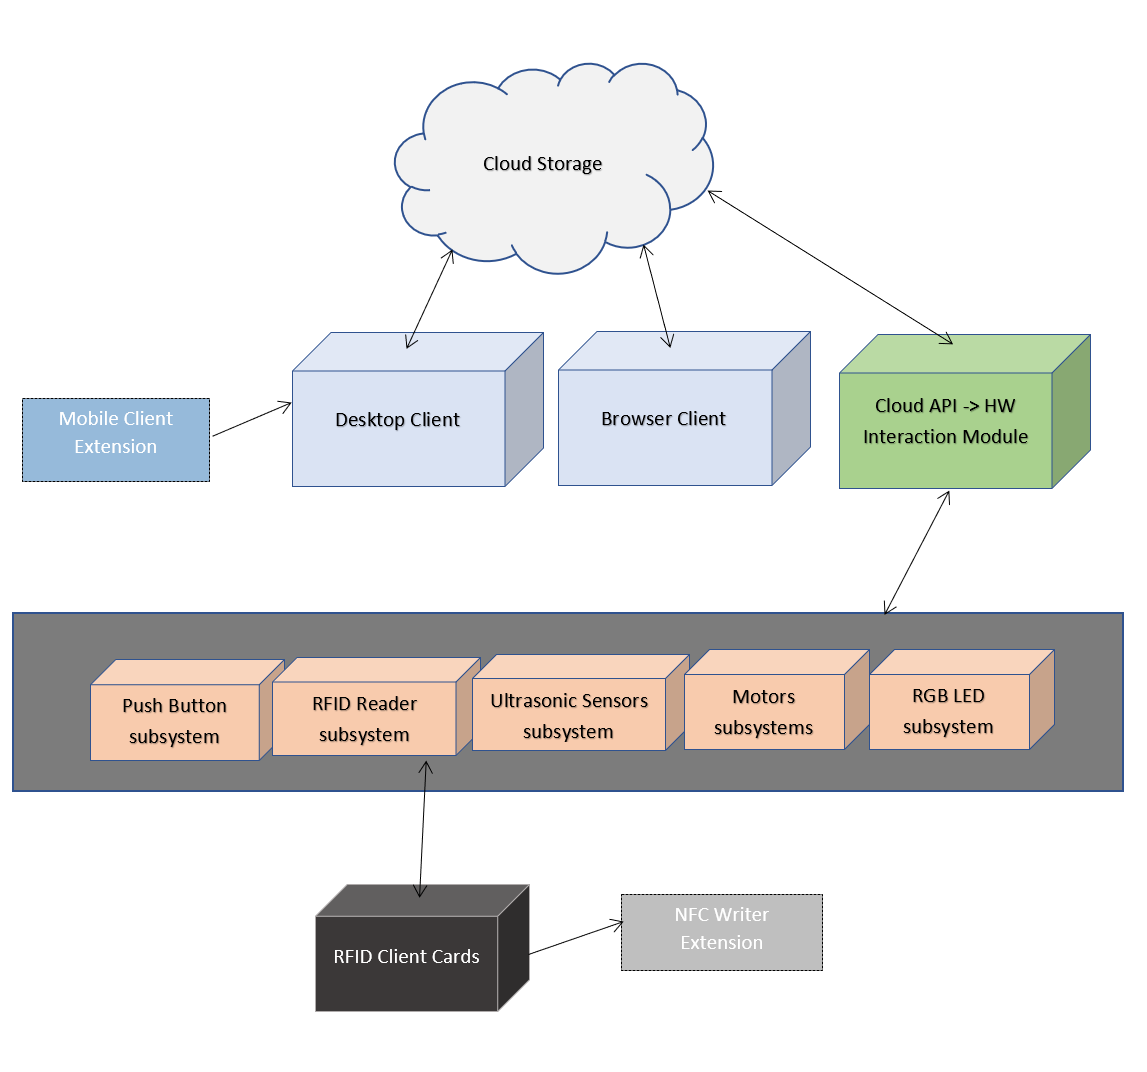
\includegraphics[scale=0.8]{SystemOverview.png}
\caption{System overview diagram}
\label{fig:system}
\end{figure}

The base modules (Push button subsystem, RFID Reader subsystem, Ultrasonic Sensors subsystem, Motors subsystem) are the actuators and the sensors of the system. The RFID Reader is able to read a user's card. The push buttons identify the products and receive input from the user in order to select one of the products. The motors start to spin based on the information received from the RPi interaction module. The ultrasonic sensors detect a product has fallen and sends a response to the motors to stop.\\\\\\

The HW Interaction Module is a Raspberry Pi that runs a python module. It interacts with the Arduino through a serial interface connection. It also communicates with the Cloud Storage through HTTP requests.\\ 

The Cloud Storage Subsystem is a Firebase module that stores user data (credit count, username, password, email), product data (stock, kcal, name, image) and the VendingHealth. client application. It also allows updating users and products.\\ 

The Dektop Client provides a UI that allows the user to view his/her credit count and view the products in the vending machine alongside the credits they would conusme.\\

The Browser Client also provides a UI that connects to the Cloud Storage and allows for an admin to change products in the vending machine and update the cloud storage with the change. It allows a new user to sign up on an RFID card and also provides the means to download the client application.

\section{Circuit design}

The hardware view of the system and the wiring of the components are depicted in Figure \ref{fig:circuit-design}.

\begin{figure}[h]
\centering
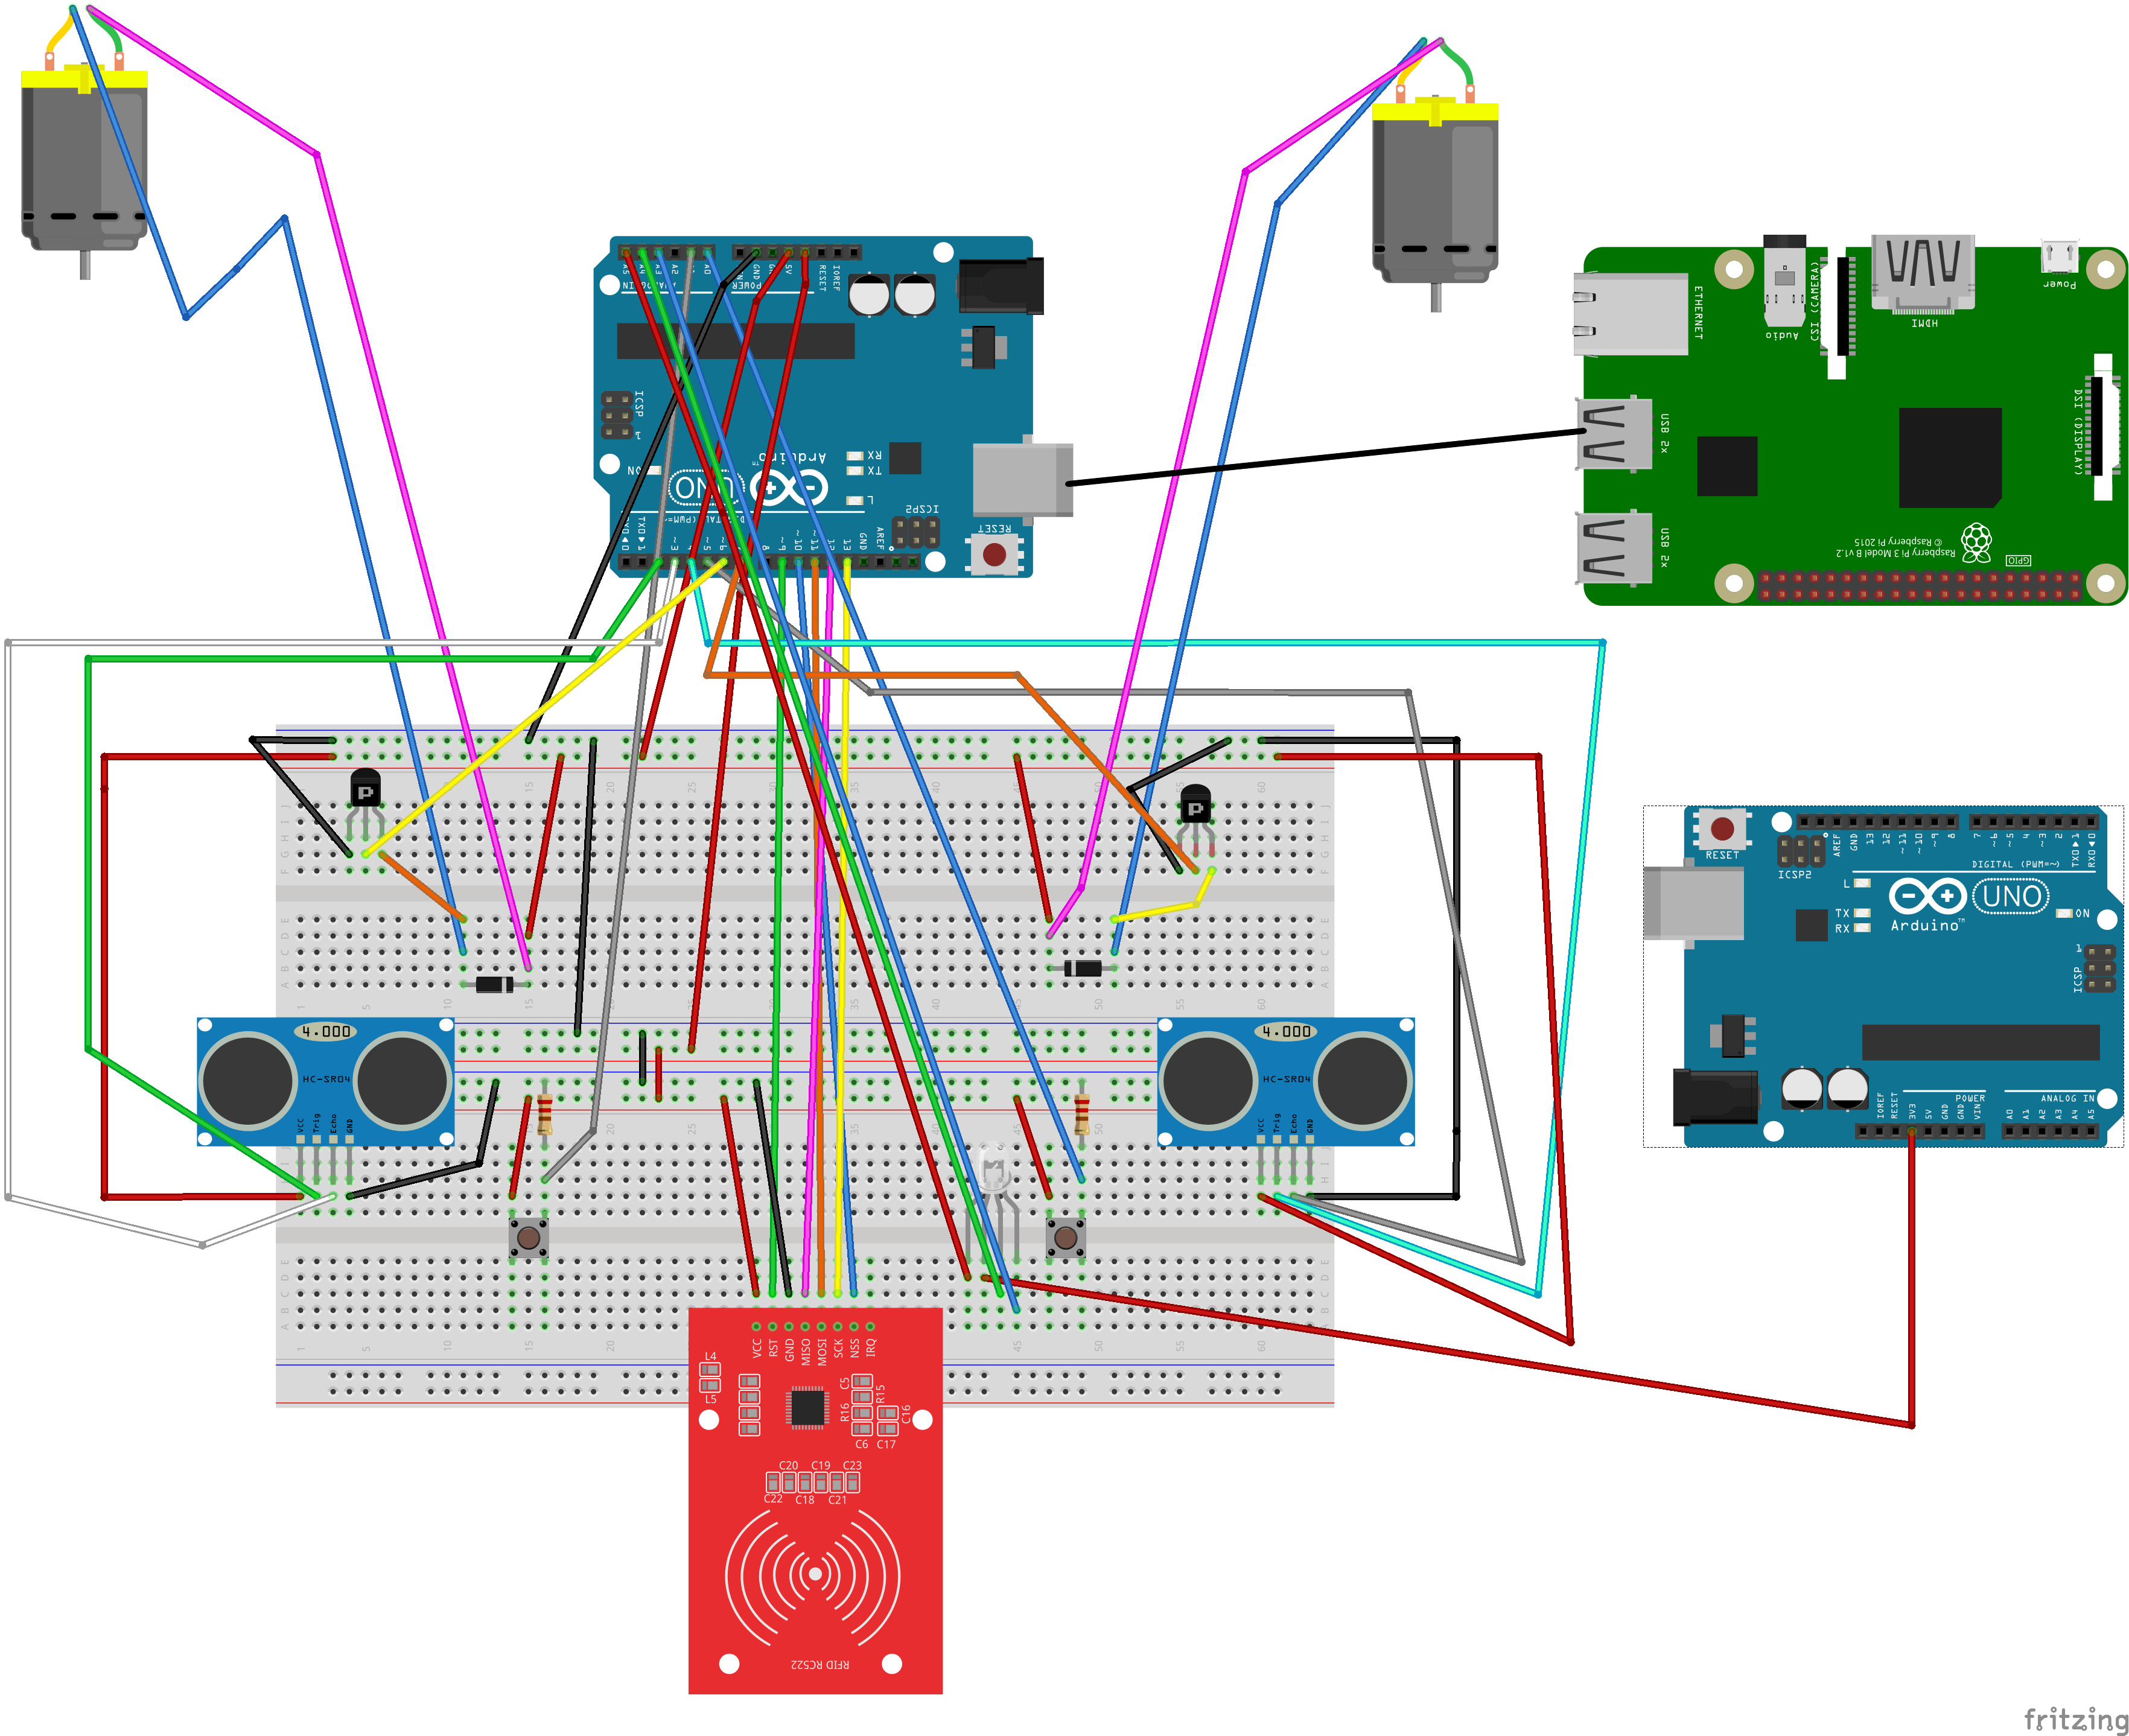
\includegraphics[scale=0.3]{CircuitDesign.png}
\caption{Circuit schematic}
\label{fig:circuit-design}
\end{figure}

Raspberry Pi 3 provides a great interface for connecting to the cloud storage and also to connect to the Arduino. It uses one of its USB ports to connect to the Arduino USB port and receive bits of information. It communicates with the cloud through the internet using HTTP GET/PATCH requests. \\

Arduino Uno provides power to its components using the 3.3V and 5V outputs. It also connects all sensors and actuators in the same environment and uses both its analog and digital pins to send impulses to all components.\\

The two HC-SR04 Ultrasonic Sensors use 2x2 of the Arduino's digital outputs for the Trig and Echo pins. The Trig pin triggers a sonic signal and then the Echo pin will transmit the received signal which represents the number of miliseconds the sound wave that was outputted traveled. The sensors are powered at 5V.\\

RFID MFRC522 is paired with two dedicated RFID cards from which it reads the tag numbers. The RFID reader is powered at 3.3V. It uses the SPI protocol to communicate with the Arduino. Ports 9 to 13 from Arduino are linked to the MISO, MOSI, SCK, IRQ, RST, NSS pins of the RFID Reader.\\

The two DC motors are powered at 5 V. They are connected to a diode and a PN2222 transistor. The diode assures that no reverse current will flow from the motor to the Arduino. The transistor allows gaining control of the motor rotation. The transistors are connected to pins 6 and 7, respectively.\\

The two push buttons are connected to the A0 and A1 pins of the Arduino and are powered at 3.3V.\\

\section{Software design}
\textit{Provide a walktrough of the most important components/modules/entities or concepts you've implemented in the software section.}\\

The software components and data flow directions are depicted in Figure \ref{fig:soft-design}. Each of these will be presented in the following subsections.\\

\begin{figure}[h]
\centering
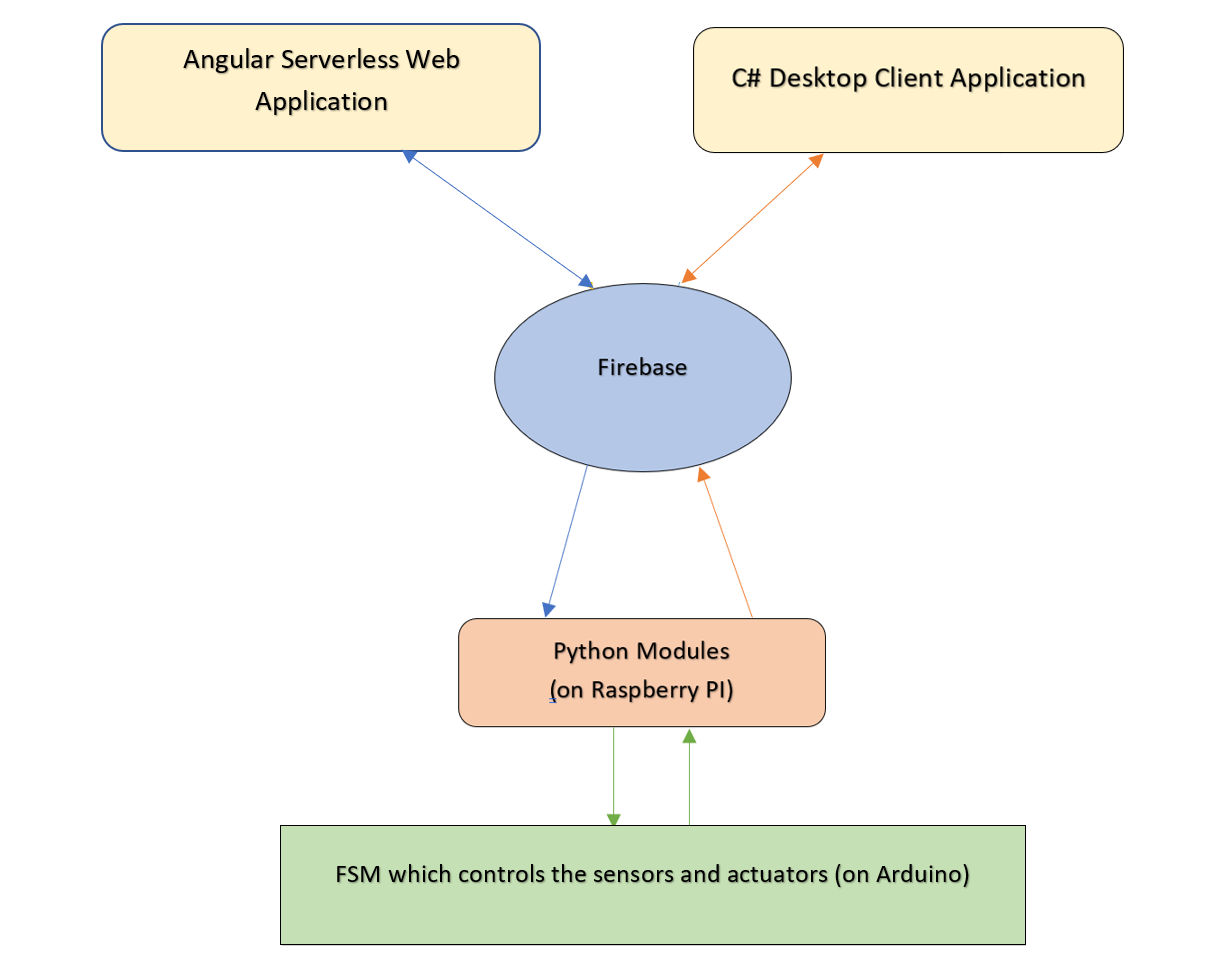
\includegraphics[scale=0.9]{SWArchitecture.png}
\caption{Software entities involved}
\label{fig:soft-design}
\end{figure}

\subsection{Arduino Modules}

\subsection{Python Modules}
\textit{You should not concentrate on providing line level descriptions, but rather class/script/module level explanations. Short code comments are strongly advised. Third party libraries should also have a brief description and a reference link.}\\

write\_firebase\_sensor.py: it retrieves the temperature and humidity tuple from DHT-22 sensor over the one-wire interface and then pushes it to Firebase every 1 second. \\

Adafruit\_DHT22 library: it provides a quick implementation of one-wire interface communication with the sensor.

\subsection{Firebase}
\textit{Describe the purpose of the service and present the specifics you are using.}\\

Firebase is a PaaS (Platform as a Service) which means it offers developers to a quick list of functionalities supported by a traditional backend.
Realtime Database simplifies storing and synchronising data between different devices in realtime using a noSQL database.

The following code section shows the initialization of the Firebase project.\\

\begin{python}
# root of the project
FIREBASE_ROOT = 'https://vendinghealth-alpha.firebaseio.com'
# init Firebase Database instance
firebase = firebase.FirebaseApplication(FIREBASE_ROOT, None)
\end{python}

\subsection{Desktop Client Application}
\textit{Explain the responsibility of some key entities contained in your Android project.}

\subsection{Browser Application}
\textit{Give a brief description of the main parts contained by the JavaScript module.}

\section{Results and further work}

The current version of the project supports the following functionalities:
\begin{itemize}
\item client implementations for retrieving product and user information stored in Firebase Database (Desktop and Web)
\item storing new products in the Firebase Database
\item allowing an admin to modify products in the Firebase Database
\item allowing users to create an account for the application and register a certain card to it
\item allowing users to download the application from the browser application\\
\end{itemize}

The following list of extensions and improvements was identified to be supported in the future:
\begin{itemize}
\item include a mobile version of the desktop application
\item extend the desktop application to Unix users
\item allow extending the number of cards that can be used with the machine 
\item improve application security (encrypt sensitive user information)
\item allow more vending machines in the Firebase database by creating a new node for each one
\end{itemize}

\newpage
\section{References}
\begin{enumerate}
\item Draw IO [last seen: May 2018], \url{https://www.draw.io/}
\item Fritzing [last seen: May 2018], \url{http://fritzing.org/}
\item Firebase Database [last seen: May 2018], \url{https://firebase.google.com/docs/database/}
\item RFID library [last seen: May 2018], \url{https://github.com/miguelbalboa/rfid}
\end{enumerate}



\end{document}
